\section{Frontend}\label{sec:impl_frontend}
Frontendová část tohoto projektu zajišťuje především komunikaci mezi uživatelem a serverem pomocí prostředí, díky kterému je tato komunikace snazší a obecně přívětivější. Serverová část očekává příchozí požadavky od této části na cesty, které byly už definovány (viz sekce \ref{sec:routes}).

V rámci této implementace (a z podstaty využitých technologií) probíhá komunikace s API (viz sekce \ref{sec:impl_backend}), které se tato část snaží poskytovat validní data. Slovo \uv{snaží} je zmíněno proto, jelikož se na ni v reálném světe nemůžeme úplně spoléhat - frontendovou část může uživatel s dostatečnými znalostmi a zkušenostmi modifikovat, čímž může i změnit způsob komunikace se serverem. To ale neznamená, že na ní nemůže probíhat jakákoliv validace a kontrola dat - frontend pro správnou funkčnost celé aplikace musí serveru ve výchozím (uživatelem nezměněném) stavu backendu poskytovat validní data - backend je ale musí preventivně validovat taky.

Uživatelské prostředí musí být připraveno tak, aby bylo příjemné k užívání a ergonomické. Zároveň by nemělo být nějak složité a přehlcené ovládacími prvky, což by mohlo uživatele od používání aplikace odradit. Dále by toto prostředí mělo uživatele \uv{vést} úkonem, který chce uživatel provést - tzn. pokud zadává neplatná data, tak ho upozornit a rozhodně počkat na opravu dat před odesláním požadavku na server. Uživatelské prostředí, které v rámci tohoto projektu vzniklo, je určeno primárně pro vykreslování ve webovém prohlížeči.

V následující části jsou popsány jednotlivé frontendové komponenty a principy, díky kterým může celá aplikace fungovat.
	
	\subsection{Obecná struktura VueJS aplikace}
	Nejprve je nutné rozebrat obecnou strukturu VueJS projektu.
	
	\begin{figure}[H]
		\centering
		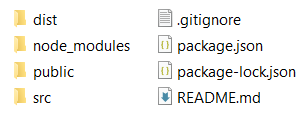
\includegraphics[width=0.6\textwidth]{img/vuejs_struktura.png} 
		\caption{Obecná struktura nově vygenerovaného VueJS projektu}
		\label{fig:vuejs_str}
	\end{figure}

	Jak můžeme na obrázku \ref{fig:vuejs_str} vidět, celý projekt je složen z mnoha složek a souborů. Podrobný rozbor všech souborů a složek není předmětem této práce, proto jsou nejdůležitější zmíněné části popsány níže jen obecně.
	
	\begin{itemize}
		\item Složka \textit{dist} obsahuje zkompilovaný kód aplikace
		\item Složka \textit{node\_modules} obsahuje závislosti a soubory přídavných balíčků, které aplikace používá
		\item Složka \textit{public} obsahuje obecně veřejné soubory (např. favicon)
		\item Složka \textit{src} obsahuje všechny soubory se zdrojovým kódem, ze kterých se poté tvoří zkompilovaný kód celé aplikace
		\item Soubor \textit{package.json} obsahuje informace o přídavných balíčcích
	\end{itemize}

	*cite https://5balloons.info/project-tour-of-vue-cli-app/*
	*cite https://stackoverflow.com/questions/22842691/what-is-the-meaning-of-the-dist-directory-in-open-source-projects*
	
	Popsaná struktura výše je standardní pro oddělenou frontendovou aplikaci. To v implementaci tohoto projektu ale neplatí, jelikož je frontend přímo zaintegrován v Laravel projektu (viz sekce \ref{sec:strukura_laravel}). Jsou zde tyto rozdíly:
	
	\begin{itemize}
		\item Složka \textit{src} je nahrazena složkou \textit{js} ve složce \textit{resources}
		\item Složka \textit{public} je umístěna v kořenovém adresáři Laravel projektu a je sloučena se složkou \textit{dist}
		\item Složka \textit{node\_modules} společně se souborem \textit{package.json} je také umístěna v kořenovém adresáři Laravel projektu
	\end{itemize}
	
	Celkovou administrativu nad celým Vue projektem poté zajišťuje modul Laravel Mix podle konfiguračního souboru webpack.mix.js. Ten je také umístěn v kořenovém adresáři projektu. *cite https://laravel-mix.com/docs/6.0/vue* Díky celému tomuto přístupu může backend i frontend běžet jako jedna aplikace na jedné doméně.
	
	Jak již bylo zmíněno, zdrojový kód, tedy nejdůležitější část frontendové aplikace, leží standardně ve složce \textit{src} - v tomto projektu ve zmíněné složce \textit{js}. Oproti běžné samostatné Vue aplikaci je zde (ve složce \textit{js}) největší rozdíl v pojmenování souborů - soubor \textit{main.js} byl přejmenován pro potřeby Laravelu na \textit{app.js}. Také se navíc v této složce nachází Laravelem vygenerovaný soubor bootstrap.js pro další konfiguraci při kompilaci. Nakonec byla kvůli nevyužití odebrána složka \textit{assets} a pro další účely přidána složka \textit{apis} (viz obrázek \ref{fig:zdroj_kod_vue_rozdily}).
	
	\begin{figure}[h]
		\centering
		\subfloat[\centering]{{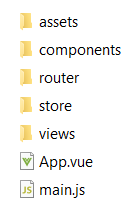
\includegraphics[height=5cm]{img/zdroj_kod_vue/src.png} }}
		\qquad
		\subfloat[\centering]{{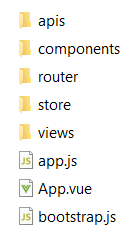
\includegraphics[height=5cm]{img/zdroj_kod_vue/js.png} }}
		\caption{Porovnání obsahu složek \textit{src} (a) a \textit{js} (b)}
		\label{fig:zdroj_kod_vue_rozdily}
	\end{figure}

	Každý soubor a složka ve zmíněném adresáři \textit{js} má určitý význam. Ty jsou představeny níže (soubor bootstrap.js byl již popsán výše). Další rozbor jednotlivých souborů ve zmíněných složkách je obsažen v dalších sekcích této práce.
	\begin{itemize}
		\item Složka \textit{apis} obsahuje prostředky pro komunikaci s API (tedy s backendem)
		\item Složka \textit{components} obsahuje všechny komponenty, které jsou využívány v celé aplikaci
		\item Složka \textit{router} obsahuje prostředky pro přesměrovávání a definování cest ve frontendové aplikaci
		\item Složka \textit{store} obsahuje nástroje pro držení dat ve webovém prohlížeči
		\item Složka \textit{views} obsahuje veškeré pohledy, na které se můžeme pomocí definované cesty dostat
		\item Soubor \textit{app.js} je kořenový soubor aplikace shromažďující všechny reference na ostatní soubory (zabaluje celou aplikaci)
		\item Soubor \textit{App.vue} je kořenová šablona, která přijímá pohledy, které poté vykresluje (tvoří aplikační kostru HTML)
	\end{itemize}
	
	\subsection{Komponenty}
	
	\subsection{Komunikace s Laravel API}
	
	\subsection{Směrovač} %%Router
	
	\subsection{Držení dat v prohlížeči} %% Store
	
	\subsection{Pohledy}
		
		\subsubsection{Přihlašování a profil}
		
		\subsubsection{Domovská stránka}
		
		\subsubsection{Formulář}
		
		\subsubsection{Tvorba formuláře}
		
		\subsubsection{Úprava formuláře}
		
		\subsubsection{Souhrn informací o formuláři}
		
		\subsubsection{Výsledky formuláře}
		
		\subsubsection{Ostatní pohledy}
		%% not found, about
